\documentclass[12pt, a4paper]{article}
\usepackage[utf8]{inputenc}
\usepackage[czech]{babel}
\usepackage[T1]{fontenc}
\usepackage{graphicx}
\usepackage{amsmath, amssymb, amsthm}
\usepackage[margin=2.5cm]{geometry}
\usepackage{url}
\usepackage{float}
\begin{document}

\begin{titlepage}
    \begin{center}
        {\large {Přírodovědecká fakulta}} \\
        \vspace{0.2cm}
        {\large Univerzita Karlova}
        
        \vspace{1.5cm}
        
\includegraphics[width=0.5\linewidth]{img/PrFUK_strom_digital_cerna.png} 
        \vfill{}
        
        {\huge\bfseries Srovnání konformních kartografických zobrazení pro zvolené území} \\
        \vspace{0.5cm}
        {\large {Matematická kartografie}} \\
        \vfill
        
        \begin{center}
            \large Teodor Sorokáč \\
        \end{center}
        \vfill{}

        \begin{center}
            \ 2. N-GKDPZ \\
            \ Praha 2026
        \end{center}
        
    \end{center}
\end{titlepage}

\newpage
\section{Zadání}

\vspace{5mm}
\subsection*{\textbf{Úloha č. 3: Srovnání konformních kartografických zobrazení pro zvolené území}}

\vspace{3mm}
Pro zvolenou dvojici států (dominantní směr, bez dominantního směru) porovnejte hodnoty délkového zkreslení u následujících kartografických zobrazení:
\vspace{3mm}

\begin{itemize}
    \item {Konformní válcové zobrazení se dvěma nezkreslenými rovnoběžkami (Mercatorovo zobrazení)}
    \[
    \begin{aligned}
    x &= R \cdot \cos(u_{0})\cos(v), \\
    y &= R \cdot \ln \tan \left(\frac{u}{2}+45^{\circ}\right).
    \end{aligned}
    \]
    
    \item {Konformní kuželové zobrazení se dvěma nezkreslenými rovnoběžkami (Lambertovo zobrazení)}
    \[
    \begin{aligned}
    \rho &= \rho_{0}\left(\frac{\tan\left(\frac{u_{0}}{2}+45^{\circ}\right)}{\tan\left(\frac{u}{2}+45^{\circ}\right)}\right)^{n}, \\
    \epsilon &= n \cdot v.
    \end{aligned}
    \]
    
    \item {Konformní azimutální zobrazení (stereografická projekce)}
    \[
    \begin{aligned}
    \rho &= 2R \cdot \tan\left(\frac{90^{\circ}-u}{2}\right), \\
    \epsilon &= v.
    \end{aligned}
    \]
\end{itemize}

\vspace{3mm}
\noindent Kartografická zobrazení pro každý stát navrhněte v obecné poloze, parametry potřebné pro výpočet odvoďte z vhodného mapového podkladu.
\vspace{3mm}

\noindent Pro navrhovaná zobrazení volte dvě nezkreslené rovnoběžky tak, aby ve středu i na okraji zájmového území byly stejné absolutní hodnoty délkového zkreslení: tj.
\[
m_{r}^{s} = m_{r}^{j} = 1 + \nu, \quad m_{r}^{r} = 1 - \nu.
\]

\vspace{3mm}
\noindent V závěru proveďte diskuzi nad dosaženými hodnotami, pokuste se tyto výsledky zobecnit a rozhodnout, které zobrazení je pro každý ze států nejvhodnější.
\vspace{3mm}

\noindent Úhlové výpočty proveďte s přesností na minuty, výpočty zkreslení na $1 \cdot 10^{-6}$.

\vspace{1cm}
\subsection*{\textbf{Hodnocení:}}

\begin{center}
\resizebox{\textwidth}{!}{
\begin{tabular}{|l|c|}
\hline
\textbf{Krok}                                                                             & \textbf{Hodnocení} \\ [0.5ex]  \hline\hline
\rule{0pt}{3ex} Srovnání kartografických zobrazení pro vybrané územní celky.                    &  20b               \\ \hline
\rule{0pt}{3ex}\textit{Exaktní výpočet dotykové rovnoběžky (válc. zobrazení).}                  &  \textit{+5b}      \\ \hline
\rule{0pt}{3ex}\textit{Kartografický pól (válc. zobrazení) s využitím analytické geometrie.}    &  \textit{+10b}     \\ \hline
\rule{0pt}{3ex}\textit{Kartografický pól (kuželové zobrazení) s využitím analytické geometrie.}  &  \textit{+15b}     \\ \hline
\rule{0pt}{3ex}\textit{Kartografický pól jako střed opsané kružnice s min. poloměrem (azim. zobrazení).} &  \textit{+10b} \\ \hline
\rule{0pt}{3ex}\textit{Ekvideformáty délkového zkreslení s vhodně zvoleným krokem (počet zobrazení).} &  \textit{+5b}   \\ \hline
\rule{0pt}{3ex}\textbf{Max celkem:}                                                       & \textbf{75b}       \\ \hline
\end{tabular}
}
\end{center}
\vspace{1.5cm}

\subsection*{Řešené bonusové úlohy}
V rámci úlohy byly vypracované následující bonusové úlohy: \textit{Exaktní výpočet dotykové rovnoběžky pro válcové zobrazení (+5b), Odvození kartografického pólu pro válcové zobrazení s využitím analytické geometrie (+10b), Odvození kartografického pólu pro kuželové zobrazení s využitím analytické geometrie (+15b), Výpočet kartografického pólu jako středu opsané kružnice s minimálním poloměrem pro azimutální zobrazení (+10b) a Generování ekvideformátů délkového zkreslení s vhodně zvoleným krokem pro všechna zobrazení (+5b).}

\newpage
\section{Popis a rozbor problému}
Cílem úlohy je srovnání vlastností jednoduchých konformních zobrazení a zhodnocení zda jsou vhodné pro zvolené území. Zda je zobrazení vhodné vychází z výpočtu délkového zkreslení $m_r$. Pro zajištění minimálního zkreslení je nutné zobrazení aplikovat v obecné poloze s určením kartografického pólu $K = [u_k, v_k]$.
\vspace{3mm}

\noindent Přechod z geografických souřadnic $(u, v)$ na kartografické $(\text{š}, d)$ se řídí transformačními rovnicemi:
\vspace{3mm}

\[
\sin \text{š} = \sin u \sin u_k + \cos u \cos u_k \cos(v - v_k)
\]
\vspace{3mm}

\[
\sin d = \frac{\cos u \sin(v - v_k)}{\cos \text{š}}
\]

\vspace{3mm}

\noindent Podmínka stejného zkreslení na okrajích a ve středu území (minimaxní kritérium) je dána vztahem:
\vspace{3mm}

\[
m_{r}^{s} + m_{r}^{r} = 2
\]

\vspace{3mm}
\noindent Pro potřeby úlohy byly vybrány dva státy, kde jeden disponuje dominantním směrem jeho území a druhý naopak nedisponuje. Proto byly vybrány státy Togo (dominantní severo-jižním směrem území) a Zimbabwe (nedominantní směr území).

\newpage
\subsection*{Válcové konformní zobrazení (Mercator)}
\vspace{3mm}
Zobrazovací rovnice v obecné poloze:
\vspace{3mm}
\[
x = R \cdot \cos(\text{š}_{0})\cos(d), \quad y = R \cdot \ln \tan \left(\frac{\text{š}}{2}+45^{\circ}\right)
\]
\vspace{3mm}
\noindent Měřítko délek $m_r$ v kartografické rovnoběžce:
\vspace{3mm}
\[
m_r = \frac{\cos \text{š}_0}{\cos \text{š}}
\]
\vspace{3mm}
\noindent Šířka nezkreslené rovnoběžky $\text{š}_0$ určená z podmínky stejného zkreslení:
\vspace{3mm}
\[
\cos \text{š}_0 = \frac{2 \cos \text{š}_{okr}}{1 + \cos \text{š}_{okr}}
\]
\vspace{3mm}
\noindent Kartografický pól $K = [u_k, v_k]$ vypočtený z ortodromy $o(P_1, P_2)$:
\vspace{3mm}
\[
\tan v_k = \frac{\tan u_1 \cos v_2 - \tan u_2 \cos v_1}{\tan u_2 \sin v_1 - \tan u_1 \sin v_2}, \quad \tan u_k = -\frac{\cos(v_1 - v_k)}{\tan u_1}
\]

\begin{figure}[H]
    \centering
    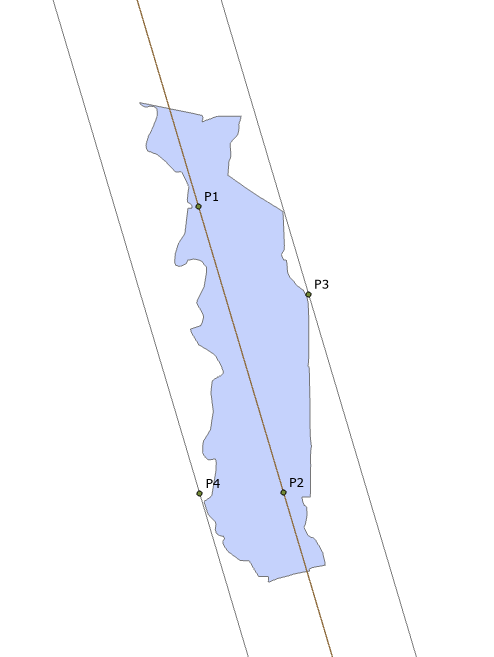
\includegraphics[width=0.7\textwidth]{img/merc_TOGO_arcgis.png}
    \caption{Hraniční linie a body pro válcové zobrazení}
\end{figure}

\begin{figure}[H]
    \centering
    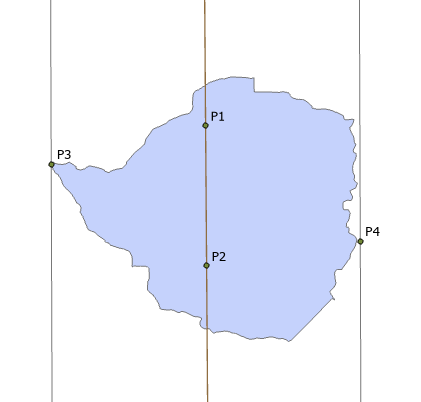
\includegraphics[width=0.7\textwidth]{img/merc_ZIMBW_arcgis.png}
    \caption{Hraniční linie a body pro válcové zobrazení}
\end{figure}

\begin{table}[H]
\centering
\begin{tabular}{|c|c|c|c|c|}
\hline
\textbf{Bod} & \multicolumn{2}{c|}{\textbf{Togo}} & \multicolumn{2}{c|}{\textbf{Zimbabwe}} \\
\hline
 & $u$ [$^\circ$] & $v$ [$^\circ$] & $u$ [$^\circ$] & $v$ [$^\circ$] \\
\hline
$P_1$ & 10.043870 & 0.469176 & -20.462362 & 29.202199 \\
$P_2$ & 7.042321 & 1.361263 & -16.865006 & 29.176271 \\
$P_3$ & 9.124304 & 1.625454 & -17.868284 & 25.216847 \\
$P_4$ & 7.028683 & 0.481770 & -19.830599 & 33.143508 \\
\hline
\end{tabular}
\caption{Souřadnice definičních bodů pro válcové zobrazení}
\end{table}

\newpage
\subsection*{Kuželové konformní zobrazení (Lambert)}
\vspace{3mm}
Konstanta kužele $c$ (případně $n$) určující míru konvergence poledníků:
\vspace{3mm}
\[
c = \frac{\log \cos \text{š}_s - \log \cos \text{š}_j}{\log \tan(\frac{\text{š}_j}{2} + 45^\circ) - \log \tan(\frac{\text{š}_s}{2} + 45^\circ)}
\]
\vspace{3mm}

\noindent Zobrazovací rovnice v polárních souřadnicích:
\vspace{3mm}
\[
\rho = \rho_{0}\frac{\tan^c(\frac{\text{š}_{0}}{2}+45^{\circ})}{\tan^c(\frac{\text{š}}{2}+45^{\circ})}, \quad \epsilon = c \cdot d
\]

\begin{figure}[H]
    \centering
    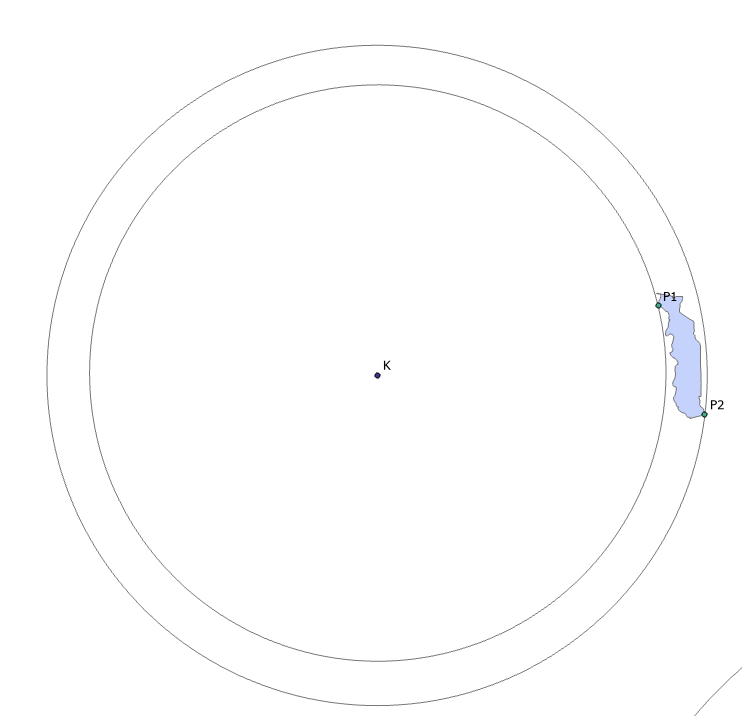
\includegraphics[width=0.7\textwidth]{img/LCC_TOGO_arcgis.png}
    \caption{Soustředné kružnice pro kuželové zobrazení}
\end{figure}

\begin{figure}[H]
    \centering
    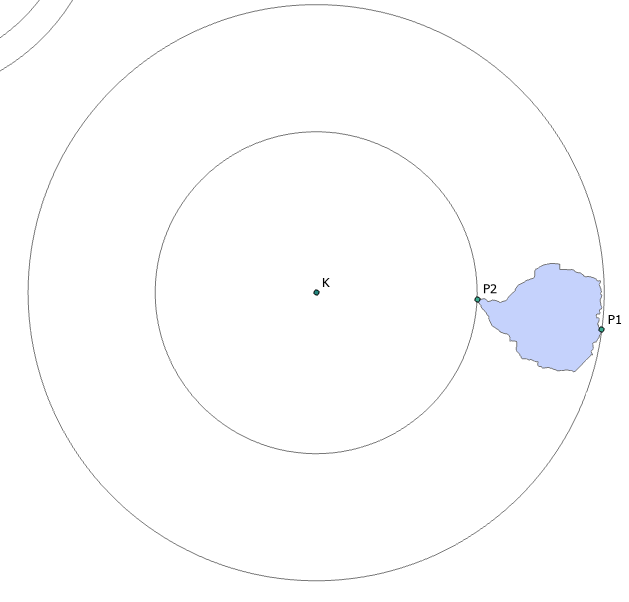
\includegraphics[width=0.7\textwidth]{img/LCC_ZIMBW_arcgis.png}
    \caption{Soustředné kružnice pro kuželové zobrazení}
\end{figure}

\begin{table}[H]
    \centering
    \begin{tabular}{|c|c|c|c|c|}
    \hline
    \textbf{Bod} & \multicolumn{2}{c|}{\textbf{Togo}} & \multicolumn{2}{c|}{\textbf{Zimbabwe}} \\
    \hline
     & $u$ [$^\circ$] & $v$ [$^\circ$] & $u$ [$^\circ$] & $v$ [$^\circ$] \\
    \hline
    $K$ & 7.836023 & -11.337276 & -17.451351 & 15.163149 \\
    $P_1$ & 10.625872 & -0.077814 & -19.762483 & 33.052730 \\
    $P_2$ & 6.277366 & 1.801811 & -17.856686 & 25.236593 \\
    \hline
    \end{tabular}
    \caption{Souřadnice definičních bodů pro kuželové zobrazení}
\end{table}

\newpage
\subsection*{Azimutální konformní zobrazení (Stereografická projekce)}
\vspace{3mm}
Zobrazovací rovnice stereografické projekce:
\vspace{3mm}
\[
\rho = c \cdot \tan\frac{\psi}{2}, \quad \epsilon = d
\]
\vspace{3mm}
\noindent kde $\psi = 90^\circ - \text{š}$. Multiplikační konstanta $\mu$ pro optimalizaci zkreslení:
\vspace{3mm}
\[
\mu = \frac{2 \cdot \cos^2(\frac{\psi_j}{2})}{1 + \cos^2(\frac{\psi_j}{2})}
\]

\begin{figure}[H]
    \centering
    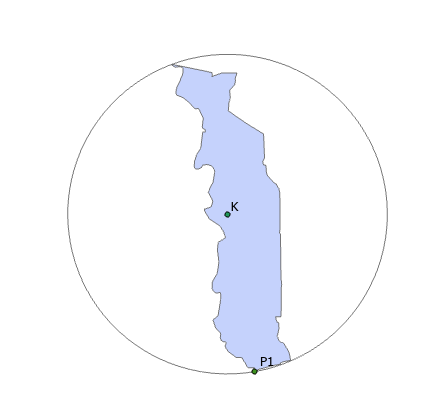
\includegraphics[width=0.7\textwidth]{img/stereo_TOGO_arcgis.png}
    \caption{Opsaná kružnice pro azimutální zobrazení}
\end{figure}

\begin{figure}[H]
    \centering
    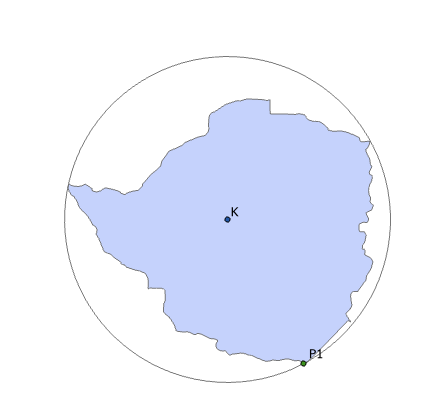
\includegraphics[width=0.7\textwidth]{img/stereo_ZIMBW_arcgis.png}
    \caption{Opsaná kružnice pro azimutální zobrazení}
\end{figure}

\begin{table}[H]
    \centering
    \begin{tabular}{|c|c|c|c|c|}
    \hline
    \textbf{Bod} & \multicolumn{2}{c|}{\textbf{Togo}} & \multicolumn{2}{c|}{\textbf{Zimbabwe}} \\
    \hline
     & $u$ [$^\circ$] & $v$ [$^\circ$] & $u$ [$^\circ$] & $v$ [$^\circ$] \\
    \hline
    $K$ & 8.681021 & 0.764245 & -18.709801 & 29.328813 \\
    $P_1$ & 6.094000 & 1.198633 & -22.401364 & 31.288830 \\
    \hline
    \end{tabular}
    \caption{Souřadnice definičních bodů pro azimutální zobrazení}
\end{table}

\newpage
\section{Výsledky a zhodnocení}
\vspace{3mm}

Pro Togo s dominantním severo-jižním směrem se jako nejvhodnější jeví zobrazení válcová a kuželová. Díky tomu, že tyto zobrazení transformují území do uzkého pásu podél optimalizované osy a tím došlo k nejlepším výsledkům a omezení maximálního délkojevného zkreslení na téměř zanedbatelnou hodnotu $\pm 0.05$ ‰. Azimutální zobrazení naopak u protáhlého tvaru generuje opsanou kružnici, která však nedokonale opisuje tvar zájmového území a tím dochází k nárůstu deformace. 
\vspace{3mm}

\begin{figure}[H]
    \centering
    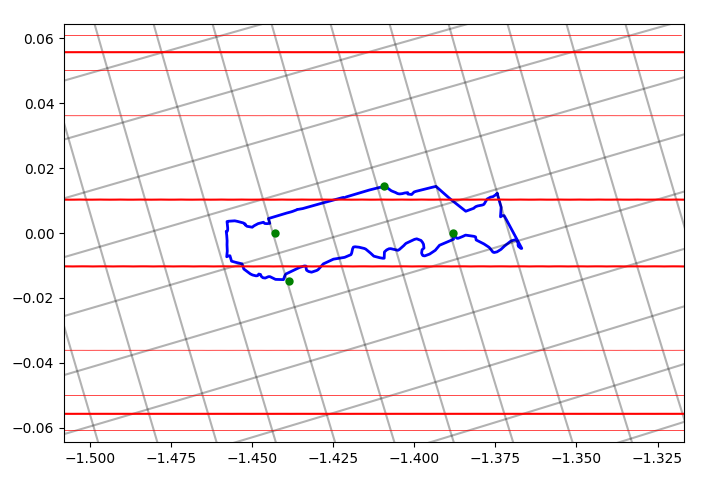
\includegraphics[width=0.7\textwidth]{img/merc_TOGO.png}
    \caption{Ekvideformáty válcového zobrazení}
\end{figure}


\begin{figure}[H]
    \centering
    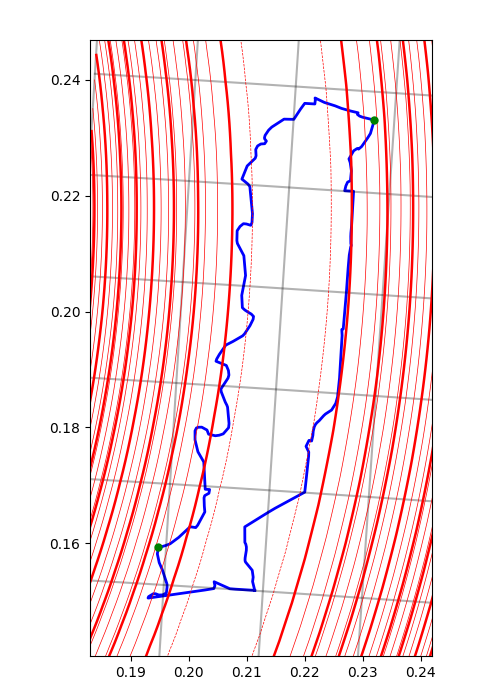
\includegraphics[width=0.7\textwidth]{img/LCC_TOGO.png}
    \caption{Ekvideformáty kuželového zobrazení}
\end{figure}


\begin{figure}[H]
    \centering
    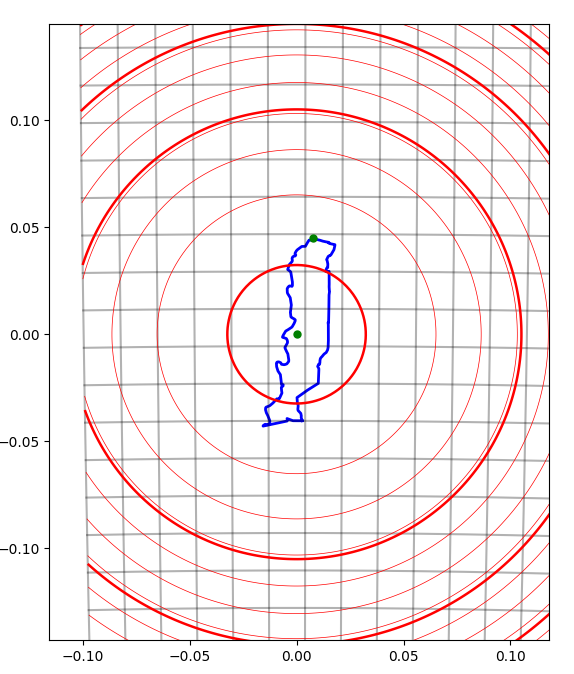
\includegraphics[width=0.7\textwidth]{img/stereo_TOGO.png}
    \caption{Ekvideformáty azimutálního zobrazení}
\end{figure}

\noindent U Zimbabwe, tedy státu bez dominantního směru území, došlo k opačnému výsledku. Kvůli tomu, že u kuželového ani válcového zobrazení nelze území zcela jednoduše vepsat do úzkého pásu, dochází tak směrem od středu k velkému navýšení zkreslení. Narozdíl od Toga, u Zimbabwe dominovalo jako nejvhodnější aziumutální zobrazení, v tomto případě stereografická projekce. Díky  koncentrickým kružnicím, ideálně pokrývá tvar území a udržuje maximální zkreslení na relativně nízkých hodnotách i na okrajích.
\vspace{3mm}

\begin{figure}[H]
    \centering
    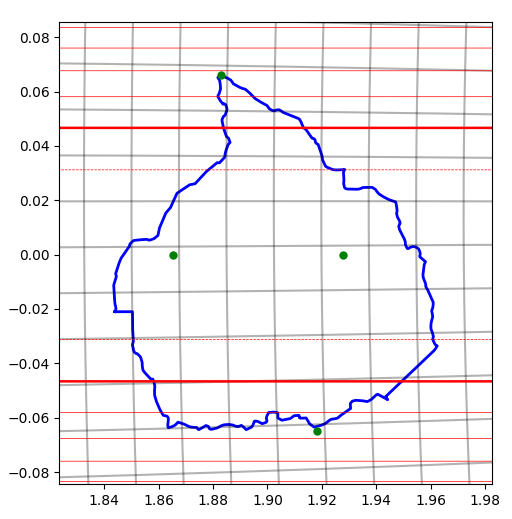
\includegraphics[width=0.7\textwidth]{img/merc_ZIMBW.png}
    \caption{Ekvideformáty válcového zobrazení}
\end{figure}


\begin{figure}[H]
    \centering
    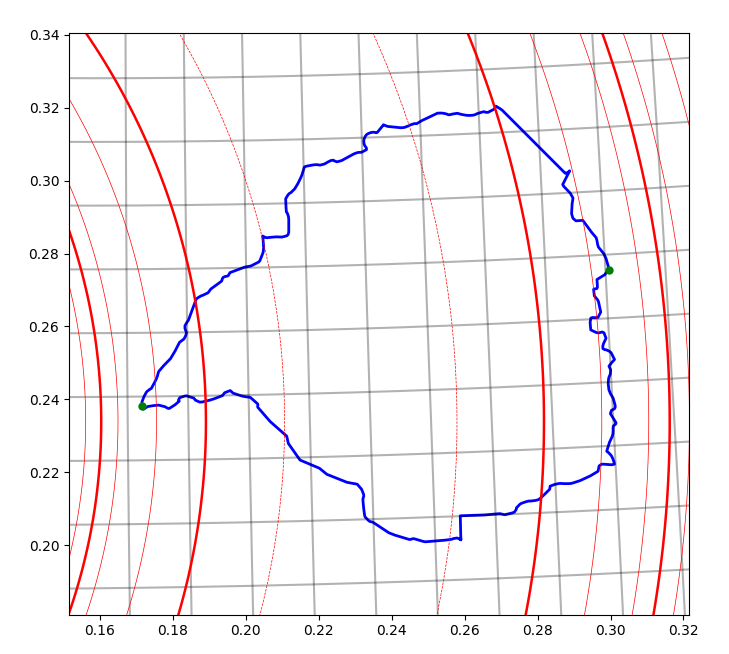
\includegraphics[width=0.7\textwidth]{img/LCC_ZIMBW.png}
    \caption{Ekvideformáty kuželového zobrazení}
\end{figure}


\begin{figure}[H]
    \centering
    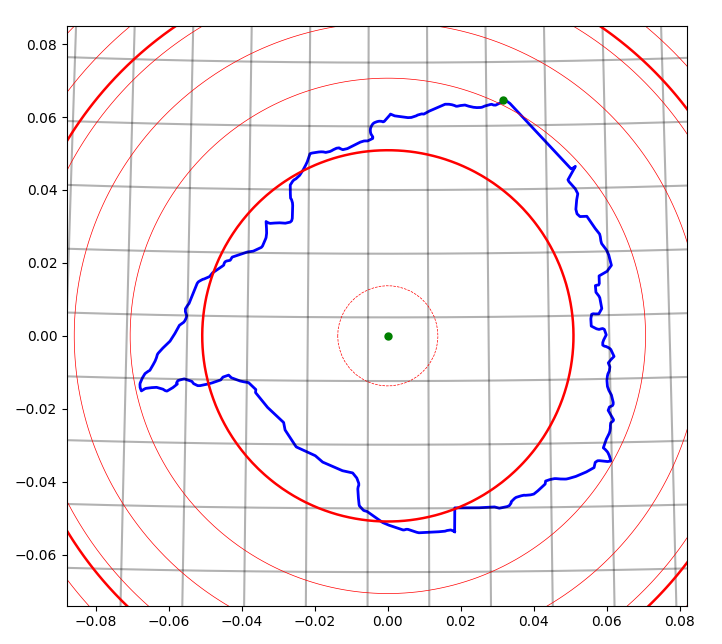
\includegraphics[width=0.7\textwidth]{img/stereo_ZIMBW.png}
    \caption{Ekvideformáty azimutálního zobrazení}
\end{figure}

\noindent Z Tabulky 4, lze potvrdit, že výběr vhodného kartografického zobrazení pro určitý typ území je zásadní. Vztah mezi tvarem a kartografickým zobrazením/projekcí je zřejmý z porovnání délkového zkreslení $m_r$.
\vspace{3mm}

\begin{table}[H]
\centering
\begin{tabular}{|c|c|c|}
\hline
 & \textbf{Togo} & \textbf{Zimbabwe} \\
\hline \hline
\textbf{bod} & \multicolumn{2}{c|}{\textbf{válcové}} \\ \hline
$P_1$ & $-0.053113$ & $-1.086101$ \\ \hline
$P_2$ & $-0.053113$ & $-1.086101$ \\ \hline
$P_3$ & $0.053113$ & $1.086101$ \\ \hline
$P_4$ & $0.054702$ & $1.013066$ \\ \hline \hline
\textbf{bod} & \multicolumn{2}{c|}{\textbf{kuželové}} \\ \hline
\textit{střed} & $-0.053423$ & $-1.080065$ \\ \hline
$P_1$ & $0.053423$ & $1.080065$ \\ \hline
$P_2$ & $0.053423$ & $1.080065$ \\ \hline \hline
\textbf{bod} & \multicolumn{2}{c|}{\textbf{azimutální}} \\ \hline
\textit{pól} & $-0.261926$ & $-0.647223$ \\ \hline
\textit{dotyková rov.} & 0 & 0 \\ \hline
$P_1$ & $0.261926$ & $0.647223$ \\ \hline
\end{tabular}
\caption{Hodnoty délkového zkreslení zaokrouhlené na $1 \cdot 10^{-6}$}
\end{table}

\newpage
\section{Seznam literatury}
\vspace{3mm}

BAYER, T. (2026): \textit{Srovnání konformních kartografických zobrazení pro zvolené území (návod na cvičení)}. Výukový materiál pro předmět Matematická kartografie, Katedra aplikované geoinformatiky a kartografie, Přírodovědecká fakulta UK [cit. 5.6.2026].


\end{document}